\documentclass[12pt]{article}
\usepackage[spanish]{babel}
\usepackage[a4paper]{geometry}
\usepackage[dvipsnames]{xcolor}
\usepackage{lipsum}
\usepackage{framed}
\usepackage{graphicx}
\usepackage{afterpage}
\usepackage{pgfplots}
\usepackage{pgf}
\usepackage{natbib}



\setlength{\parskip}{12pt}
\setlength{\parindent}{0cm}
\renewcommand{\arraystretch}{1.2}
\setcounter{secnumdepth}{4}

\geometry{top=2.5cm, bottom=2.5cm, left=2.5cm, right=2.5cm}
\begin{document}



\renewcommand{\listtablename}{Índice de tablas}
\renewcommand{\tablename}{Tabla}

\definecolor{light-gray}{gray}{0.87}  

\begin{titlepage}
\hspace*{-3.5cm}
    \begin{minipage}{\textwidth}
        \vspace{-2.5cm}
        \begin{center}
    

            
\includegraphics[width=\paperwidth]{LogoEHU.PNG}
        \end{center}
    \end{minipage}

\vspace{1cm}

\hspace{-3.1cm}
\noindent\fcolorbox {light-gray}{white}{

    \parbox{\paperwidth}{
     \begin{center}
     \large Gradu amaierako lana /Trabajo fin de grado
    \\
             \large Ingenieritza Kimiko gradua/ Grado en Ingeniería Química

\end{center}
    }
    }


\vspace{0.8cm}

\noindent\hspace*{-2.5cm}%
\colorbox{light-gray}{\begin{minipage}{\paperwidth}%

    \vspace{1cm}

    \color{RoyalBlue}
    \centering\Large\textbf{ LanarenAAAA izenbgkasduhjygkfgaksdggkjhasdgurua / Título del trabajo}
    \\
    \centering\textmd{ Lanaren azpitituloa / Subtitulo del trabajo}


    \vspace{6cm}\mbox{}
  \end{minipage}
}

\begin{flushright}
 Egilea/ Autor/a:
\\
Andoitz Campo Pérez
\\
Zuzendariak/Directores/as:
\\
Asier Aranzabal Maiztegi
\\
XXX XXX                      
\\
\end{flushright}

\begin{center}
\noindent\fcolorbox {white}{white}{

    \parbox{11cm}{
         \begin{center}
    \footnotesize © 2021, se puede proteger poniendo nombre y apellido/izen abizenak ezarriz babes zaitezke edo lizentzia CC batekin babestu / o con una licencia CC
    \\
   \small http://es.creativecommons.org/blog/licencias/

        \end{center}
    }
    }
\end{center}

\hspace{-3.2cm}
\noindent\fcolorbox {light-gray}{white}{
    \begin{minipage}[]{1000pt}

        \parbox{\paperwidth}{
            \begin{center}
    
                 Leioa, 2021eko XXXren XXa / Leioa, XX de XXX de 2021

            \end{center}
        }
    \end{minipage}
}
\end{titlepage}

\tableofcontents

\newpage 

%%%%%%%%%%%%%%%%%%%%%%%%%%%%%%%
%Hemendik aurrera hasi lana idazten%
%%%%%%%%%%%%%%%%%%%%%%%%%%%
\section{INTRODUCCIÓN}


\subsection{CONTEXTO}
El sector de la automoción, engloba una gran variedad de industria  y servicios dedicados a servirla. Se estima que la aportación total de las actividades relacionadas con este sector asciende a un 11\% del PIB lo que lo convierte en la segunda industria manufacturera que mas  ingresos aporta después de el 18,8\% del PIB que posee  la industria agroalimentaria española (Díaz y Montoriol Garriga, 2021). Esta cifra se puede ver coincide con la carta emitida por el presidente de la ANFAC en su informe anual, donde s

El  este sector, él vehículo de propulsión autónoma, es generalmente utilizado para el transporte de pasajeros y mercancías. Entre los componentes que lo forman, se encuentran las cubiertas o neumáticos, encargados de transmitir la energía del motor al asfalto, y convertirla en energía cinética.asd.:w


La producción de la industria manufacturera de cubiertas, posee una clara tendencia al alza en los últimos años, como se observa en la Figura \ref{fig:global_prod_evo}. Bridgestone es el mayor fabricante de neumáticos a nivel mundial, compartiendo mercado con Michelin \citep{rodgers2020tire}.  Existe una gran competencia, como se puede apreciar en la Figura \ref{fig:brand_revenue}. Según los valores de la propia empresa, la clave para permanecer líder en su sector, son la continua innovación y la calidad superior de sus productos.

\begin{figure}[h]
    \begin{center}
        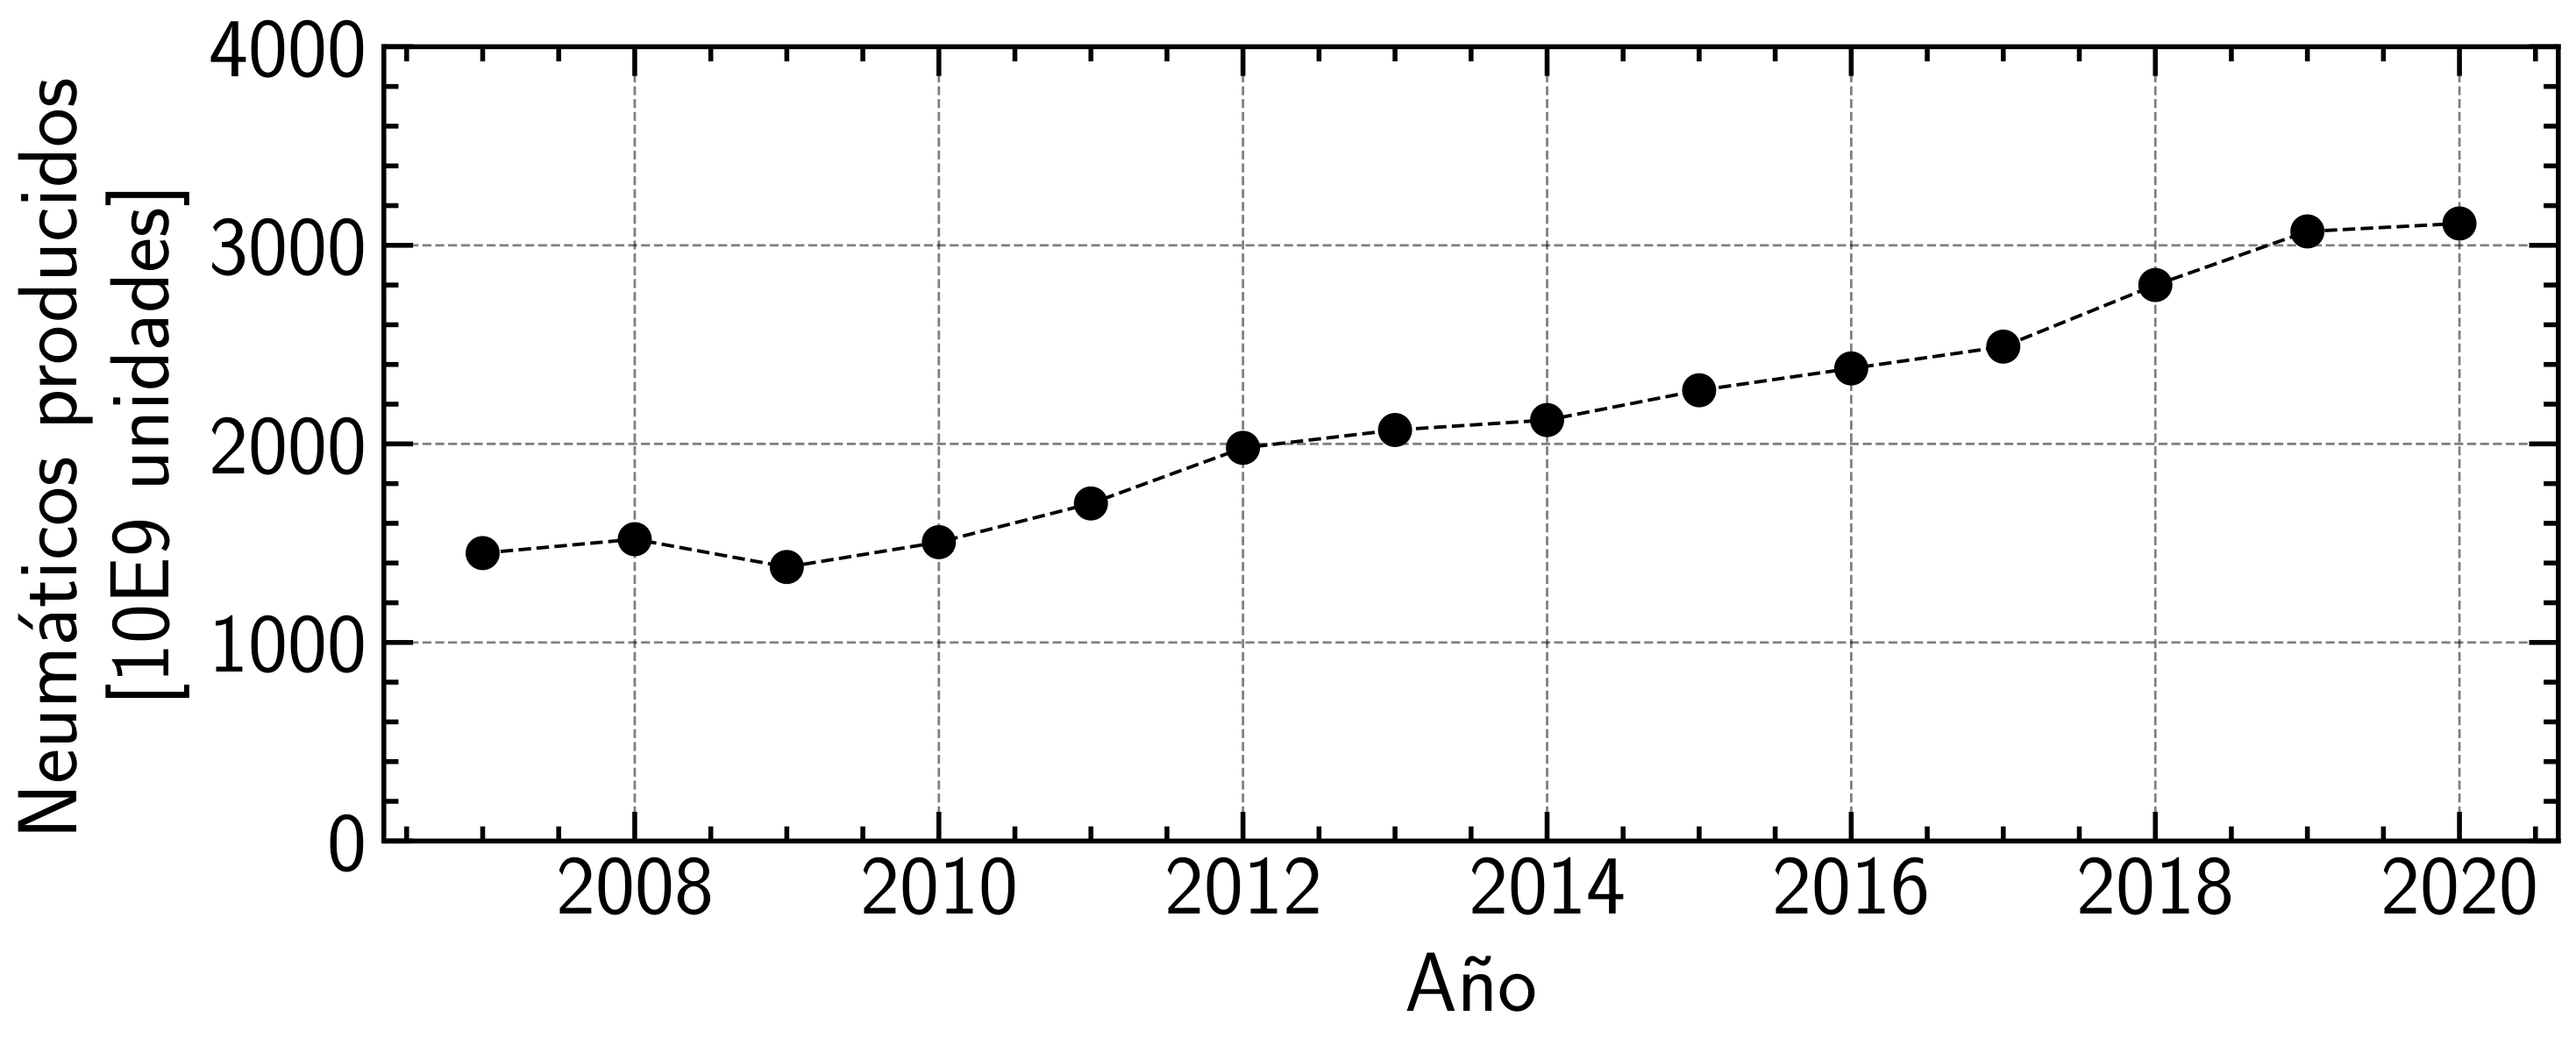
\includegraphics[width=\textwidth]{global_prod_evo.PNG}    
    \end{center}
    \caption{Evolución de la producción mundial de cubiertas.}
    \label{fig:global_prod_evo}
\end{figure}

\begin{figure}[h]
    \begin{center}
        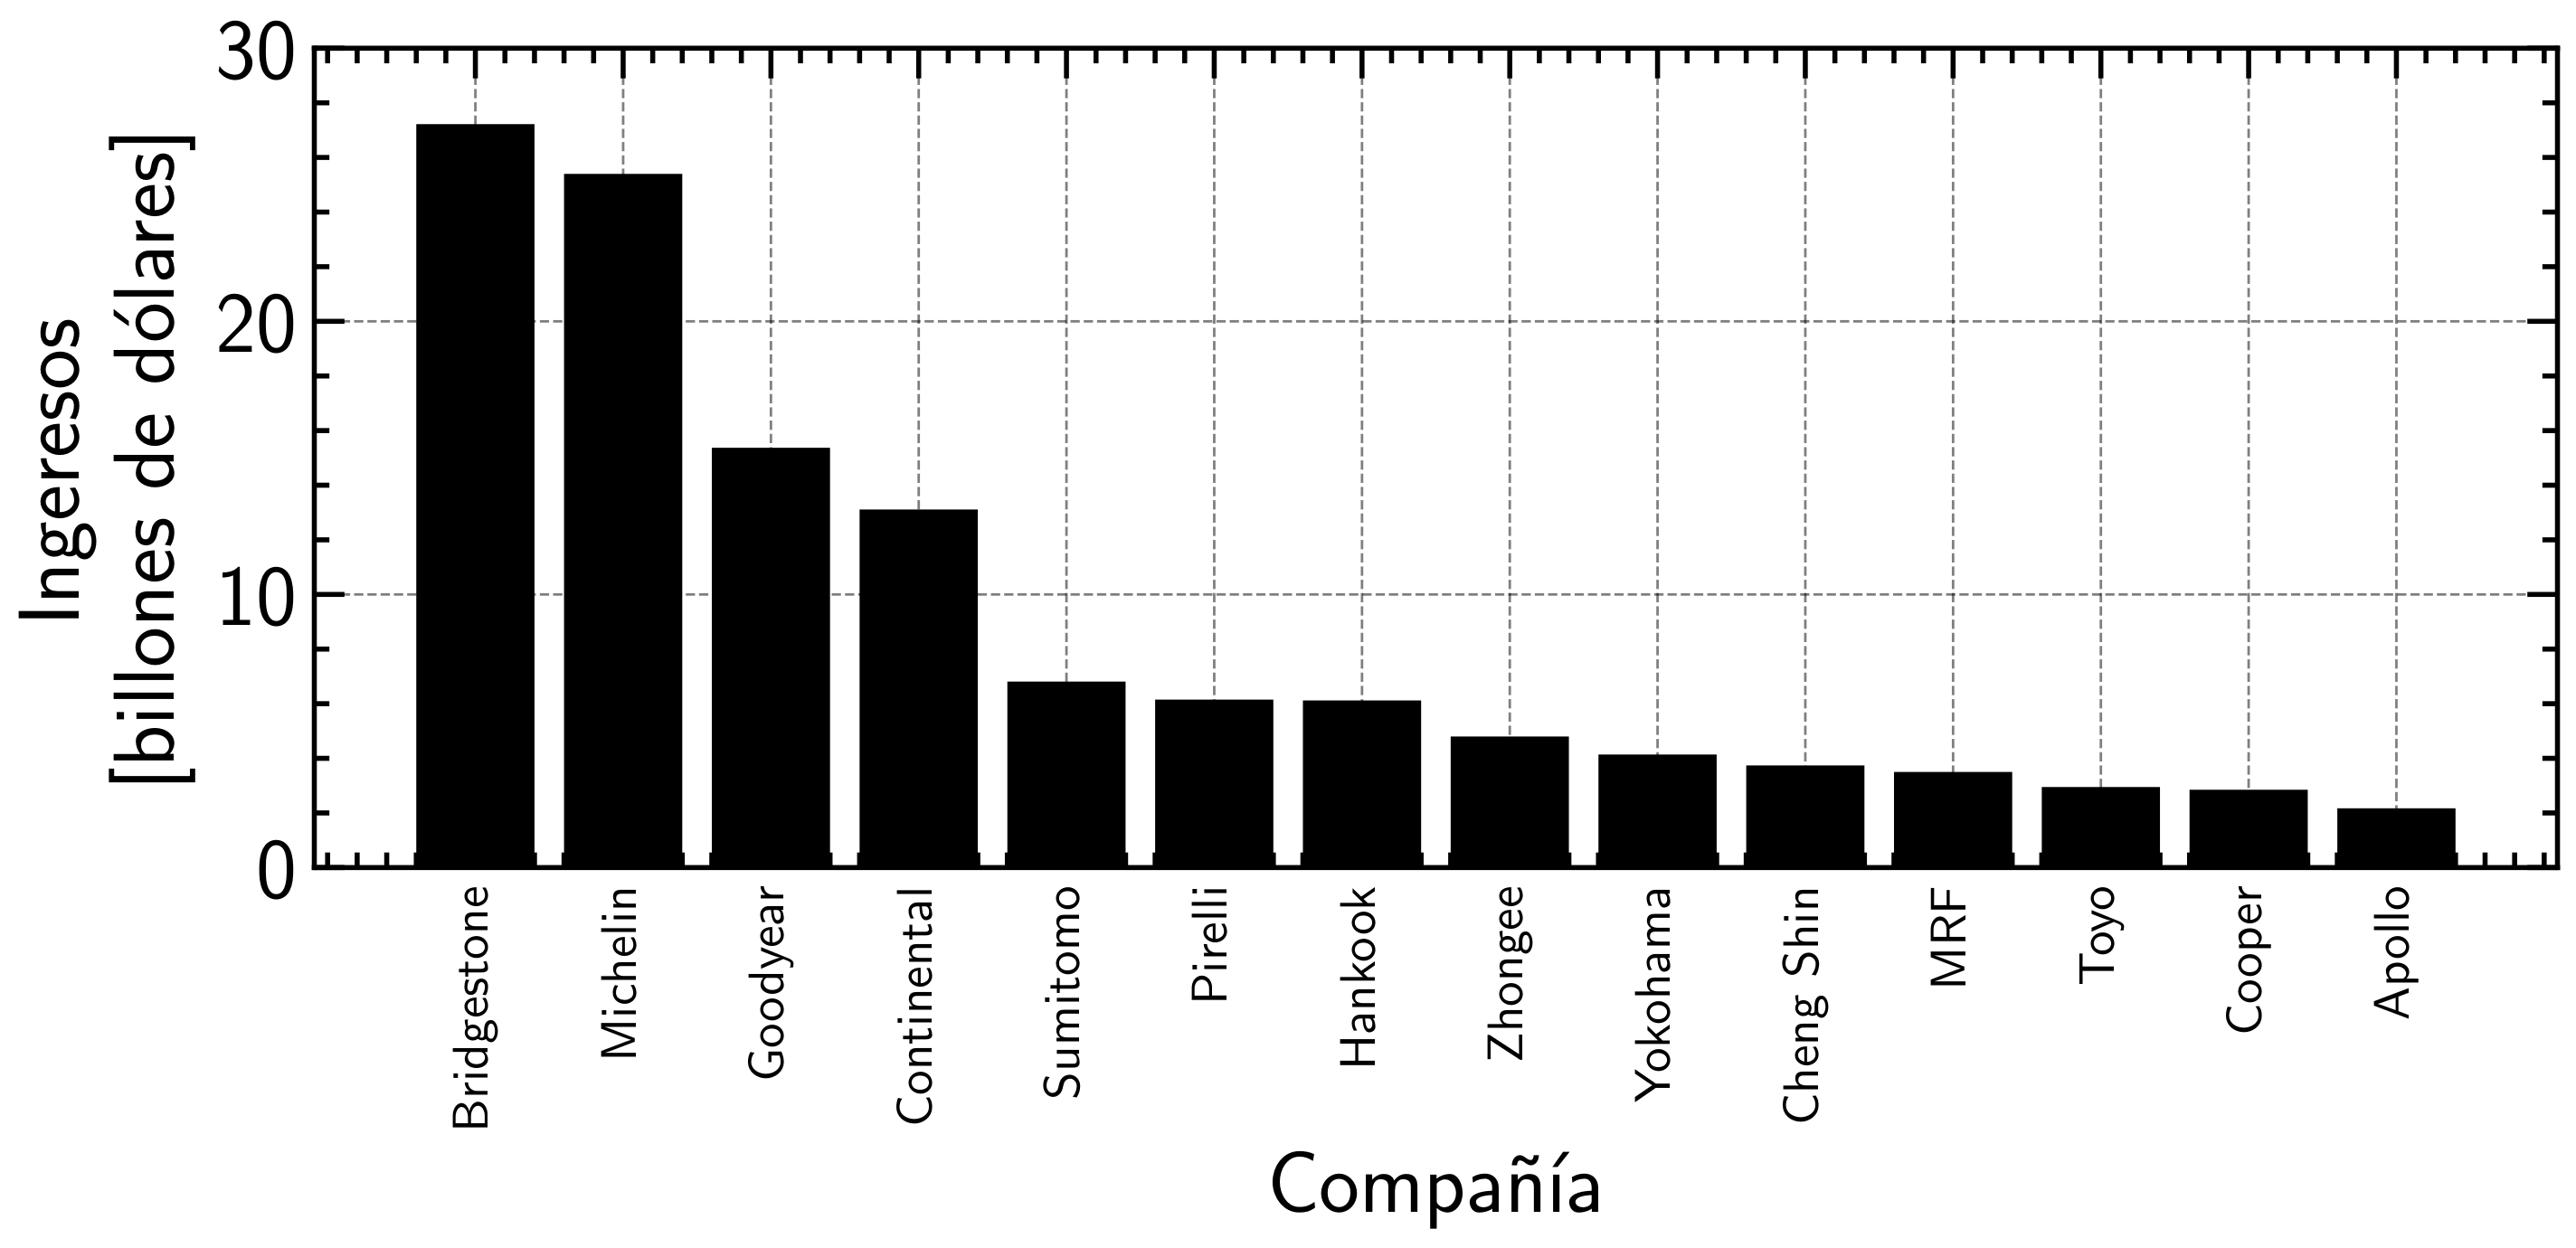
\includegraphics[width=\textwidth]{brand.revenue.PNG}    
    \end{center}
    \caption{Ingresos de los fabricantes de neumáticos más relevantes en 2019.}
    \label{fig:brand_revenue}
\end{figure}

La tarea de evaluar los productos experimentales y la Conformidad de la Producción (CoP) recae en gran medida sobre el Laboratorio de Evaluación del Producto (LEP). Esto se traduce en una correlación positiva entre la inversión en el LEP y los ingresos anuales percibidos por la compañia.

La planta de Basauri esta experimentando un incremento de un 16\% en la producción este 2022 esperando alcanzar hasta un incremento del 26\% en 2023. El LEP que previamente ya se encontraba al límite de su capacidad, debe afrontar esta demanda ascendente. Sin una clara fuente de información en la que basar la iniciativa de ampliación del departamento, una inversión precipitada, puede acarrear resultados inesperados en el rendimiento del laboratorio, y una gran pérdida económica.

Con el objetivo de tomar la decisión correcta, se ha decidido, a propuesta del autor de este trabajo, realizar una simulación estocástica que abarca cada rutina ejecutada en el LEP. Esta simulación acoge los principios de la simulación Monte Carlo, extensamente conocida a nivel mundial por su aplicación en apuestas y juegos de azar. El método de Simulación de Eventos Discretos (DES), adhiere complejidad a su ascendiente enfocándose en el detalle de los procesos. Mediante una representación  granular de la realidad traducida a un modelo computacional, es capaz de obtener respuestas a los cambios de variable en sistemas complejos.
 
\subsection{OBJETIVOS}

El objetivo principal de esta trabajo es el de proveer a la planta de Bridgestone Basauri con la información necesaria para tomar la decisión de realizar una inversión más conveniente sobre la ampliación del laboratorio, en un futuro cercano.

Para lograr el objetivo final se deberán completar los siguientes subobjetivos:

\begin{itemize}
  \item Modelar los procesos del laboratorio de acuerdo a los fundamentales de una DES, obteniendo un modelo ajustado a la realidad.
  \item Definir las variable independientes relevantes en el proceso, que posteriormente se introducirán en el sistema.
  \item En caso de ser posible obtener datos de las duraciones de los procesos modelados, ajustando sus distribuciones empíricas a la distribución estándar que mejor se ajuste. En caso contrario, proceder con la mejor estimación posible provista por los técnicos expertos.
  \item Definir las variables dependientes que otorgara el sistema a la salida. Estas variables serán los indicadores o KPIs usados para evaluar el rendimiento del sistema.
  \item Desarrollar un programa de simulación en el entorno de Python usando la librería Simpy que emule los distintos escenarios propuestos en la metodología.
  \item Comparar los KPIs obtenidos y proponer el escenario más óptimo a la organización para su posterior implementación.
\end{itemize}

\subsection{RESUMEN}

\section{MARCO TEÓRICO}
\subsection{LEAN}
\subsection{SECTOR DE LA AUTOMOCIÓN}

El sector de la automoción, engloba una gran variedad de industria y servicios dedicados a servirla. Sin ella concebir el mundo tal y como lo conocemos hoy en día resulta difícil. Desde el diseño e innovación, pasando por la manufactura de las materias primas y componentes de un vehículo, el ensamblaje de todo este material, hasta su venta y su uso en el comercio y el transporte, genera una gran cadena de valor añadido vital para las economías. En un análisis publicado por el banco Caixabank, se estima que la aportación total de las actividades relacionadas con este sector asciende a un 11% del PIB lo que lo convierte en la segunda industria manufacturera que mas ingresos aporta después de el 18,8% del PIB que posee la industria agroalimentaria española (Díaz y Montoriol Garriga, 2021). Esta cifra se puede ver contrastada en la carta emitida por el presidente de la ANFAC en su informe anual, donde se expone un PIB del 10% (ANFAC, 2022).
 
La industria automovilística, siendo claramente uno de los motores de la economía, pude dividir sus beneficios entre tres principales orígenes: la fabricación y esamblado de vehículos, los prestamos y financiaciones asociados a su venta y la fabricación de las piezas que lo componen. Entre las pizas utilizadas en los vehículos terrestres habituales, se encuentran las cubiertas, esenciales a la hora de transmitir la potencia del motor a la calzada. El mercado de las cubiertas ha ido manteniendo una tendencia al alza desde el año 2015 hasta el comienzo de la pandemia del Covid19 en el que alcanzo un volumen de 2000 millones de unidades anuales producidas. Durante este periodo, su producción aumentó en un 4,08\%, crecimiento que se vio prácticamente anulado por los acontecimientos del 2020 y congelación que sufrió la economía. Con la reactivación del mercado, la producción mundial ha repuntado, y se espera que para el 2026 la producción supere las 2700 unidades anuales (RubberWorld, 2021).

Englobar todos los tipos de cubiertas puede ser una decisión apropiada para apreciar la bastedad de este sector, pero si por algo se caracterizan las cubiertas es por su diseño. El diseño de los pneumaticos se vé claramente condicionado a las aplicaciones donde se utilizará cambiando drásticamente sus características dependiendo del vehículo en el que se montará, la ruta que seguirá este vehículo y las condiciones climáticas que deba soportar.Es por esto que este producto fabricado a partir del caucho, debería clasificarse según el uso final que se le da. Un buen esquema podría ser el propuesto por la European Tyre and Rim Technical Organisation (ETRTO) que regula las características de los pneumaticos para distintos sectores (ETRTO, 2022). A continuación la traducción de la lista mencionada en el estándar:

\begin{itemize}
	\item Cubiertas para automóvil de pasajeros
	\item Cubiertas para vehiculos comerciales
	\item Cubiertas para equipo agrónomo
	\item Cubiertas para ciclos y ciclomotores
	\item Cubiertas para uso industriales y carretillas elevadoras – Pneumaticas
	\item Cubiertas para uso industriales y  carretillas elevadoras – Solidas
	\item Cubiertas para equipo de movimiento de tierra

\end{itemize}

Particularmente, este trabajo pondrá su foco en la categoría de cubiertas para vehículos comerciales, ya que esta acoge las cubiertas de transporte de mercancías y de transporte publico que se fabrican en la planta de Basauri.

\subsubsection{Transporte y logística}

La posibilidad del comercio como lo conocemos hoy en día no existiría sin el transporte y la logística. Según Díaz, “Los sistemas de transportes y logística han estado estrechamente relacionados a las transformaciones históricas del comercio” (Díaz, 2014).

Según la literatura, la logística representa el cumulo de actividades que asegura la disponibilidad de los productos correctos, en cantidades correctas a los clientes correctos (Raja, 1998). Es el paso intermedien la cadena de valor entre la producción y el consumo. El transporte, en cambio, sería únicamente la actividad de mover el producto a su destino dentro del concepto de la logística. Este comparte espacio junto con otras actividades como, el control de inventario, el almacenamiento, el tratamiento del material dentro de las instalaciones etc. Entre estas actividades, entorno al 40\% del coste, se asocia al transporte.

La realidad del transporte europeo puede ser observada analizando las bases de datos publicadas por la Eurostat. Según sus datos, el total del transporte de bienes anual por carretera rondaría los 14.000 millones de toneladas anuales, como se puede observar en la tabla 1. Esta cuota del mercado, se habría mantenido sobre ¾ del transporte de bienes dentro del comercio intraeuropeo, respecto a otros métodos e transporte como se puede observar en la figura 1.

Debido a que la demanda del transporte no solo abarca el comercio con mercancías, es interesante a su vez analizar la extensión de el sistema de transporte de pasajeros. En los resumen de 2019 de la Uinon Europea se aprecia que el volumen total de pasajeros por kilometro recorrido fue de 3,314 millones. El sector está claramente dominado por los coches de pasajeros con una cuota del 85 , seguido por el transporte en autobuses y similares que supondría el 12\%, dejando lo restante a las motocicletas. 

\begin{table}[h!]
\centering
\begin{tabular}{|c|cccccccccc|}

	\hline
	AÑO & 2010 & 2011 & 2012 & 2013 & 2014 & 2015 & 2016 & 2017 & 2018 & 2019\\ 
	\hline
	MTA & 15046 & 14997 & 13963 & 13772 & 13989 & 14123 & 14247 & 14659 & 14656 & 14998\\ 
	\hline
	
\end{tabular}

\caption{Evolución de transporte de mercancía por carretera en MTA: Millones de Toneladas Año.}
\label{table:1}

\end{table}

\begin{figure}
    \begin{center}
        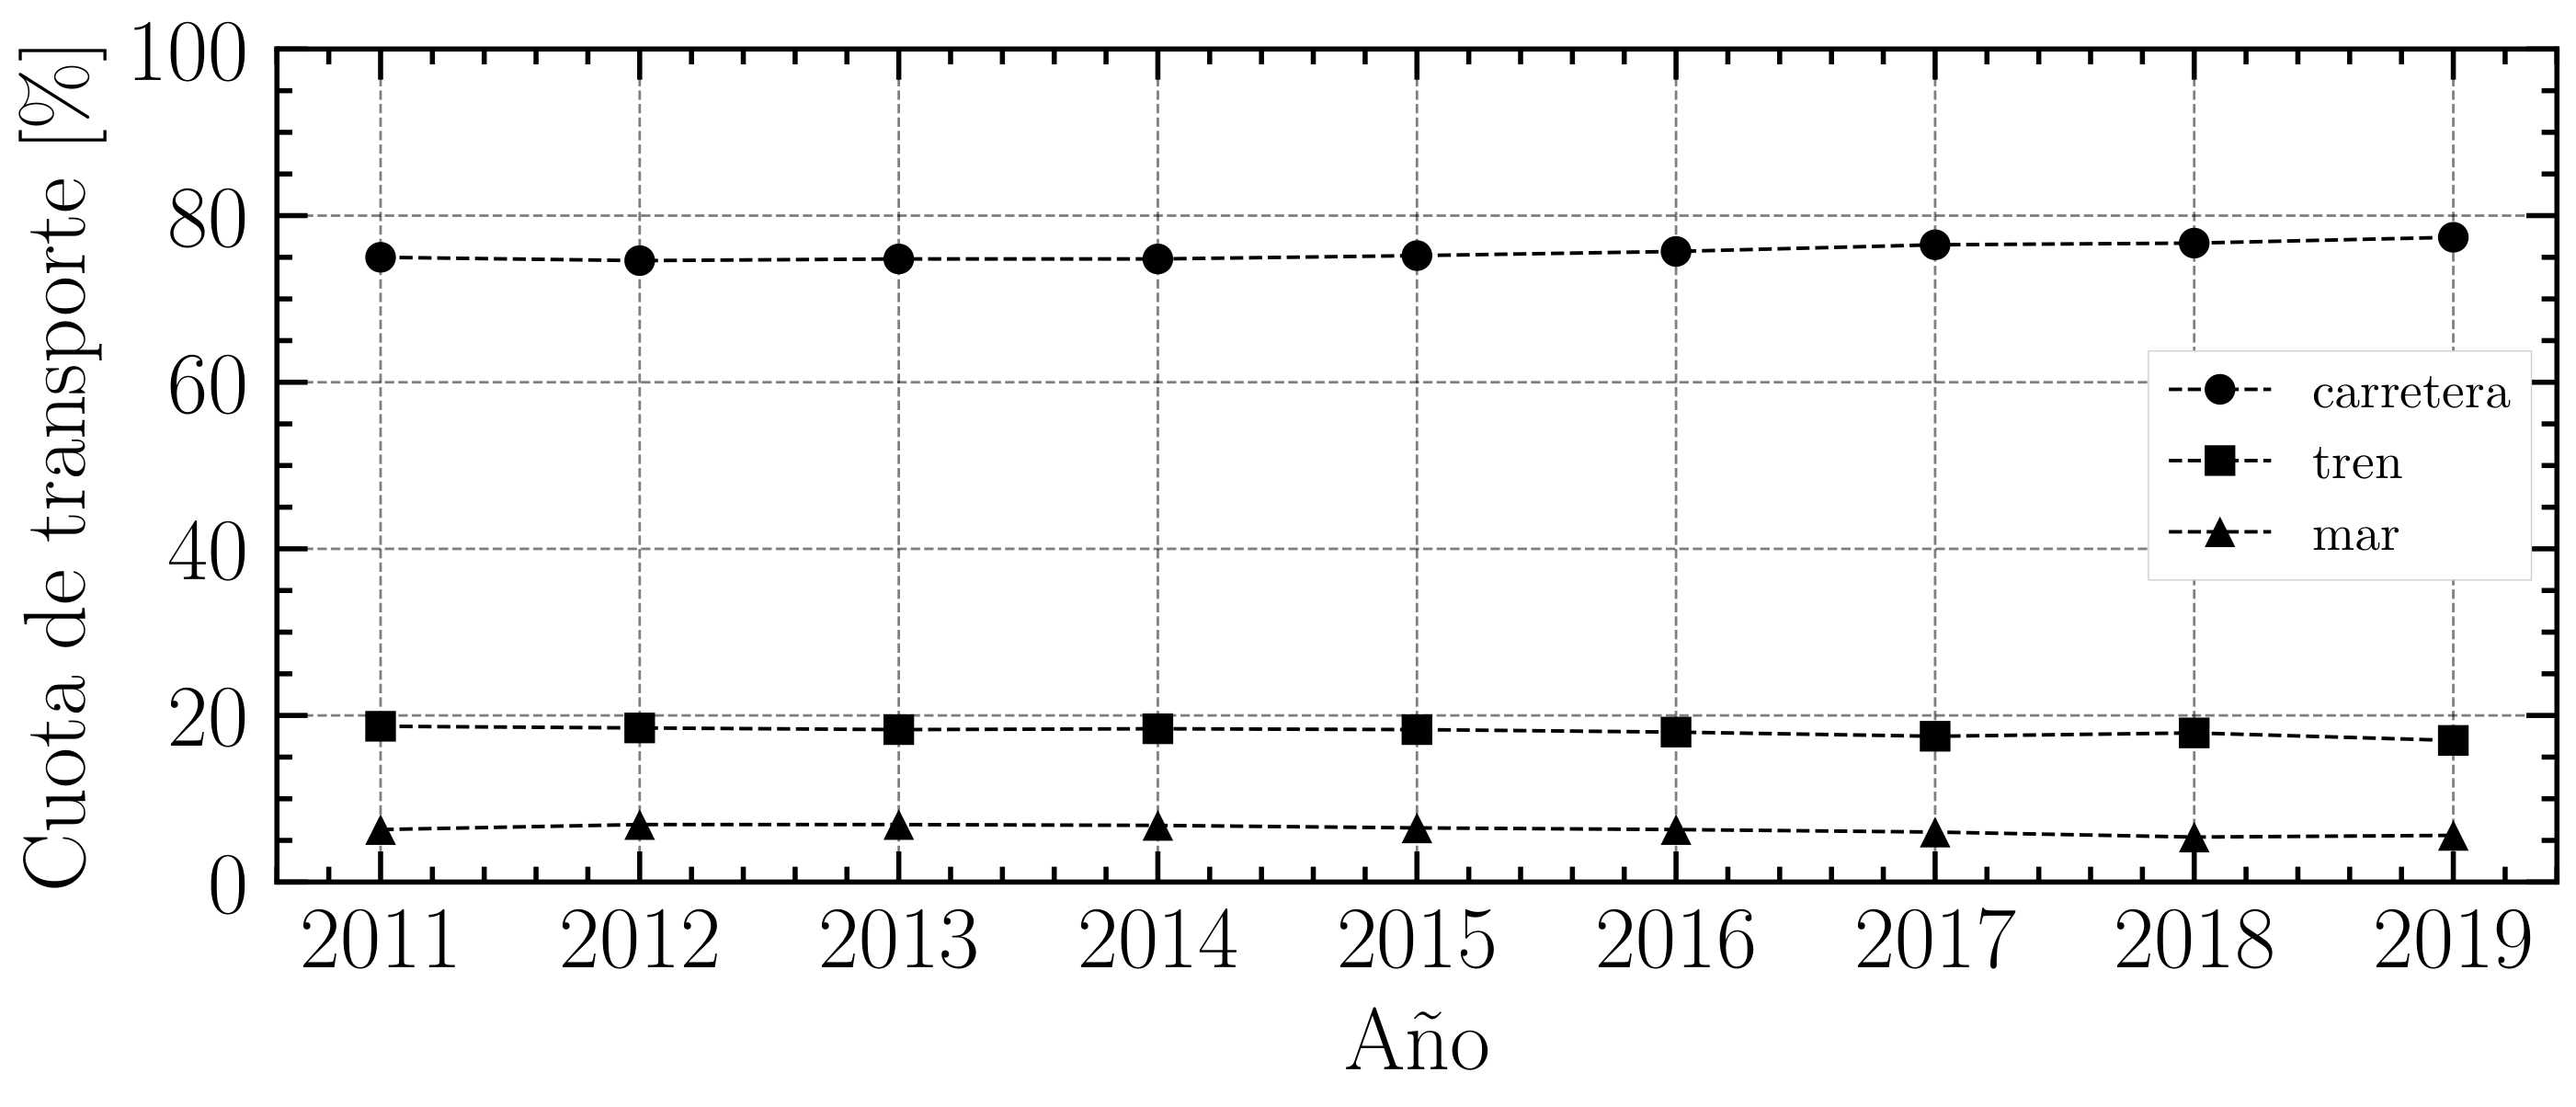
\includegraphics[width=\textwidth]{freight_transport_methods_evolution.PNG}    
    \end{center}
    \caption{Evolución de la cuota de transporte por cada tipo de transporte.}
\end{figure}

\subsubsection{Cubiertas TBR y LTR}

\paragraph{Construcción}

\paragraph{Proceso de manufacturación}

\paragraph{Control de calidad en el LEP}

\subparagraph{Quality control Endurance Drum (QCED)}

\subparagraph{Rolling Resistance (RR)}

\subparagraph{Analisis de sección y Huella (CSA  + FP)}

\subparagraph{FSMV 119 (DOT)}

\subparagraph{Bead Fatigue (BF)}


\subsection{SIMULACIÓN DE EVENTOS DISCRETOS}
Con el avance tecnológico experimentado desde los inicios de la computación, nuevas maneras de resolución de problemas han surgido que antaño se calificaban cómo poco viables e incluso imposibles. La capacidad de calculo y el diseño de inteligencias artificiales nos ha brindado la oportunidad de afrontar problemas que con metodos clasicos serían increiblemente dificiles de modelar.La simulación hoy en día es una de las tres metodologías consolidadas, en el ambito cientifico e ingenieril para la resolución de problemas \citep{banks1998handbook}. Siendo esta descrita como "La técnica de último recurso" por el autor \citep{garzia1986discrete}, debido a la intensa demanda computacional que requería en aquellos tiempos, el transcurso de los años ha minimizado esta desventaja.

Diversos autores describen la simulación de la siguiente manera:
\begin{itemize}
\item ``Una simulación es el establecimiento de un modelo logico-matemático de un sistema y la manipulación experimental de este en un computadoora digital\citep{pritsker1974gasp}"

\item ``La simulación es proceso de diseñal el modelo de un sistema real y realizar experimentos con este modelo con el propósito de, o bien, entender el comportamiento del sistema, o evaluar distintas estrategias (dentro de los límites impuestos por un criterio o conjunto de criterios) para la operación del sistema \citep{shannon1976systems}''.

\item ``Una simulación es la imitación de el modo de operación de un proceso real o sitema durante el transcurso del tiempo'' \citep{banks1999introduction}.
\end{itemize}

Como se puede observar, el termino modelo es concurrente en el ámbito de la simulación. En palabras de \citep{banks1998handbook}, ``Un modelo es la representación del sistema simulado". Según el autor la virtud de un modelo radica en su complejidad, siendo necesario un balance que de lugar a una representación suficientemente fidedigna, sin complicarlo en exceso. Aquellos factores que no influyan lo suficiente en los resultados de la simulación deberían ser eliminados al solo demorar el proceso de desarrollo.

El modelo, por tanto constituye la base de la simulación, define las variables, y criterios para las decisiones tomadas en la simulación. Mientras que la mayoría de modelos matemático y estadísticos representan las variables independientes y dependientes de forma explicita, definiendo los pasos intermedios mediante relaciones matemáticas, un Sistema de Eventos Discretos se enfoca en la representación de los componentes internos \citep{banks1998handbook}. En palabras del propio autor, la recreación de los componentes internos y sus interacciones son debe llegar a desarrollarse hasta cumplir con los objetivos del caso de estudio.

Una Simulación de Eventos Discretos funciona de manera que el sistema va alternando su estado durante el transcurso del tiempo, sucediendo ``eventos'' entre dichos cambios \citep{varga2001discrete}. Estos eventos son instantáneos, es decir que el tiempo que toman para ser realizados es nulo. Durante el evento no habrá ocurrido nada de interés, salvo el cambio en el estado del sistema desde el estado previo al evento hasta el posterior. Una sencilla representación de esta idea pude ser observada en la figura \ref{fig:diagrama_basico_DES}, donde el sistema representado es un coche que posee 3 estados posibles. Los estados se van sucediendo mientras avanza el tiempo, ocurriendo el cambio en los eventos.

\begin{figure}[h]
    \begin{center}
        \includegraphics{ejemplo_simple_DES}    
    \end{center}
    \caption{Representación de el cambio de estado en una DES, los rectángulos representan el estado del sistema mientras que las flechas indican el suceso de un evento instantáneo.}
    \label{fig:diagrama_basico_DES}
\end{figure}

\subsubsection{Términología y funcionamiento en una DES}\label{TF_DES}

Para describir detalladamente este tipo de simulaciones, es necesario definir previamente algunos conceptos. Los siguientes conceptos han sido extraidos del libro publicado por \citep{banks1998handbook} y la documentación de la librería Simpy programada en Python colgada en su página web oficial:

\begin{itemize}
\item Las variables del estado del sistema son el conjunto de información necesaria para observar el comportamiento del sistema. Estas definen el estado del sistema en el tiempo. Su determinación varía de proyecto a proyecto, pero siempre deben escogerse con los objetivos presentes. Un ejemplo de estas es el momento de inicio y fin de un subproceso.
\item Las entidades hacen referencia a objetos en el modelo. Hay dos tipos de entidades, las dinámicas, las cuales avanzan por el sistema, y las estáticas, que dan servicio a las primeras. Siguiendo con la temática automovilística, una entidad dinámica podría ser un coche, mientras que una estática podría ser la estación de la gasolinera o un hueco en el aparcamiento. Estas entidades pueden poseer atributos, como el color de un coche o el tamaño de su deposito. Dependiendo del objetivo de la simulación, algunos atributos de la entidad serán relevantes, y deberán ser incluidos en la simulación.
\item Un recurso es una entidad que provee de servicio a una entidad dinámica. Los recursos pueden servir a varias entidades simultáneamente, y de manera inversa, una entidad puede solicitar varios tipos de recurso y cantidades. Si la demanda de una entidad no se satisface, ésta entrara en una cola, a la espera de la liberación del recurso. Si la entidad toma el recurso, ésta lo mantendrá ocupado durante la duración del subproceso. Los recursos pueden tener varios estados como el de disponible, ocupado, averiado, en reparación...
\item Una actividad es un periodo de tiempo cuya duración es conocida  previamente al inicio de la actividad. La duración de la actividad puede ser determinada de varias maneras mediante; una constante, una distribución estadística, un resultado de una ecuación, un archivo, o una decisión basada en el estado del sistema. Esto supone que el inicio y el fin de la actividad es conocido, lo que facilita la computación de las entidades en cola.
\item Una demora es un periodo de espera indefinido antes del comienzo de una actividad. Este depende de la ejecución de el resto de actividades prioritarias, por lo que en el comienzo de la cola no se puede determinar cuanto durara la espera.
\item Un evento se considera el principio o fin, tanto de una actividad como de una demora. Por lo tanto, un evento, es la consecuencia de las actividades y demoras.
\end{itemize}

Considerando todos estos conceptos, las entidades del sistema compiten entre ellas por el uso de los recursos, si estos no se encuentran disponibles, quedan a la espera de poder solicitarlos. Tanto las actividades como las demoras reclaman estas entidades durante los intervalos entre eventos, siendo liberadas para el siguiente paso una vez finalizado el periodo. Una Simulación de Eventos Discretos, puede describirse como el avance de una entidad a través de las actividades que modelan un proceso real. Este avance es activado mediante el transcurso de tiempo virtual dentro de la simulación.

\subsubsection{Exposición de un caso ficticio usando una DES}
Con el objetivo de ilustrar los conceptos descritos en la sección \ref{TF_DES} y demostrar la capacidad de resolución de problemas de la DES, se ha procedido a emular un caso práctico. Tomado como referencia el modelo descrito en la figura \ref{fig:diagrama_basico_DES}, se ha redactado la siguiente problemática.

Supongase una jornada laboral que comienza desde el amanecer y que finaliza al atardecer del mismo día. Durante este periodo, varios individuos deciden tomar el coche para desplazarse a distintos lugares, entre los cuales la mayoría ira al trabajo en horarios similares, mientras que los demás serán conductores ocasionales que usen su vehículo a lo largo del día repartidos de manera equitativa. De esta población una fracción deseará repostar en la gasolinera más cercana a el parking donde estacionaran sus vehículos.

El comportamiento del sistema descrito, puede ser emulado mediante una DES aplicando las variables expuestas en la tabla y el diagrama de la figura \ref{fig:simulation_example_diagram}.

\begin{figure}
    \begin{center}
        \includegraphics{simulation_example_diagram}
    \end{center}
    \caption{Modelo de ejemplo para demostrar el funcionamiento de una DES.}
    \label{fig:simulation_example_diagram}
\end{figure}

\subsubsection{Análisis DAFO}

\subsubsection{Etapas de desarrollo de una DES}

\begin{figure}
    \begin{center}
        \includegraphics{simulation_diagram}
    \end{center}
    \caption{Esquema del proceso de desarrollo de una DES.}
    \label{fig:simulation_diagram}
\end{figure}


\section{METODOLOGÍA}
\section{DESARROLLO}
\section{CONCLUSIONES}

\newpage 

\bibliographystyle{elsarticle-harv}
\bibliography{mybibfile}
\end{document}
